\documentclass{sigchi}

% Use this section to set the ACM copyright statement (e.g. for
% preprints).  Consult the conference website for the camera-ready
% copyright statement.

% Copyright
\CopyrightYear{2021}
%\setcopyright{acmcopyright}
\setcopyright{acmlicensed}
%\setcopyright{rightsretained}
%\setcopyright{usgov}
%\setcopyright{usgovmixed}
%\setcopyright{cagov}
%\setcopyright{cagovmixed}
% DOI
\doi{https://doi.org/10.1145/3313831.XXXXXXX}
% ISBN
\isbn{XXX-X-XXXX-XXXX-X/21/05}
%Conference
\conferenceinfo{CHI'21,}{May 8--13, 2021, Yokohama, Japan}
%Price
%\acmPrice{\$15.00}

% Use this command to override the default ACM copyright statement
% (e.g. for preprints).  Consult the conference website for the
% camera-ready copyright statement.

%% HOW TO OVERRIDE THE DEFAULT COPYRIGHT STRIP --
%% Please note you need to make sure the copy for your specific
%% license is used here!
% \toappear{
% Permission to make digital or hard copies of all or part of this work
% for personal or classroom use is granted without fee provided that
% copies are not made or distributed for profit or commercial advantage
% and that copies bear this notice and the full citation on the first
% page. Copyrights for components of this work owned by others than ACM
% must be honored. Abstracting with credit is permitted. To copy
% otherwise, or republish, to post on servers or to redistribute to
% lists, requires prior specific permission and/or a fee. Request
% permissions from \href{mailto:Permissions@acm.org}{Permissions@acm.org}. \\
% \emph{CHI '16},  May 07--12, 2016, San Jose, CA, USA \\
% ACM xxx-x-xxxx-xxxx-x/xx/xx\ldots \$15.00 \\
% DOI: \url{http://dx.doi.org/xx.xxxx/xxxxxxx.xxxxxxx}
% }

% Arabic page numbers for submission.  Remove this line to eliminate
% page numbers for the camera ready copy
% \pagenumbering{arabic}

% Load basic packages
\usepackage{balance}       % to better equalize the last page
\usepackage{graphics}      % for EPS, load graphicx instead 
\usepackage[T1]{fontenc}   % for umlauts and other diaeresis
\usepackage{txfonts}
\usepackage{mathptmx}
\usepackage[pdflang={en-US},pdftex]{hyperref}
\usepackage{color}
\usepackage{booktabs}
\usepackage{textcomp}
\usepackage{lipsum}

% Some optional stuff you might like/need.
\usepackage{microtype}        % Improved Tracking and Kerning
% \usepackage[all]{hypcap}    % Fixes bug in hyperref caption linking
\usepackage{ccicons}          % Cite your images correctly!
% \usepackage[utf8]{inputenc} % for a UTF8 editor only

% If you want to use todo notes, marginpars etc. during creation of
% your draft document, you have to enable the "chi_draft" option for
% the document class. To do this, change the very first line to:
% "\documentclass[chi_draft]{sigchi}". You can then place todo notes
% by using the "\todo{...}"  command. Make sure to disable the draft
% option again before submitting your final document.
% \usepackage{todonotes}

% Paper metadata (use plain text, for PDF inclusion and later
% re-using, if desired).  Use \emtpyauthor when submitting for review
% so you remain anonymous.
\def\plaintitle{Lifestyle and study equipment changes during distance learning}
\def\plainauthor{First Author, Second Author, Third Author, Fourth Author}
\def\emptyauthor{First Author, Second Author, Third Author, Fourth Author}
\def\plainkeywords{distance learning; student; home office; study environment; work environment; motivation; pandemic; health; }
\def\plaingeneralterms{Documentation, Standardization}

% llt: Define a global style for URLs, rather that the default one
\makeatletter
\def\url@leostyle{%
  \@ifundefined{selectfont}{
    \def\UrlFont{\sf}
  }{
    \def\UrlFont{\small\bf\ttfamily}
  }}
\makeatother
\urlstyle{leo}

% To make various LaTeX processors do the right thing with page size.
\def\pprw{8.5in}
\def\pprh{11in}
\special{papersize=\pprw,\pprh}
\setlength{\paperwidth}{\pprw}
\setlength{\paperheight}{\pprh}
\setlength{\pdfpagewidth}{\pprw}
\setlength{\pdfpageheight}{\pprh}

% Make sure hyperref comes last of your loaded packages, to give it a
% fighting chance of not being over-written, since its job is to
% redefine many LaTeX commands.
\definecolor{linkColor}{RGB}{6,125,233}
\hypersetup{
  pdftitle={\plaintitle},
% Use \plainauthor for final version.
%  pdfauthor={\plainauthor},
  pdfauthor={\emptyauthor},
  pdfkeywords={\plainkeywords},
  pdfdisplaydoctitle=true, % For Accessibility
  bookmarksnumbered,
  pdfstartview={FitH},
  colorlinks,
  citecolor=black,
  filecolor=black,
  linkcolor=black,
  urlcolor=linkColor,
  breaklinks=true,
  hypertexnames=false
}

% create a shortcut to typeset table headings
% \newcommand\tabhead[1]{\small\textbf{#1}}

% End of preamble. Here it comes the document.
\begin{document}
\title{\plaintitle}
\numberofauthors{4}
\author{
  \alignauthor{Author One\\
    \affaddr{for Submission}\\
    \affaddr{}\\
    \email{}
    }\\
  \alignauthor{Author Two\\
    \affaddr{for Submission}\\
    \affaddr{}\\
    \email{}
    }\\
  \alignauthor{Author Three\\
    \affaddr{for Submission}\\
    \affaddr{}\\
    \email{}
    }\\
  \alignauthor{Author Four\\
    \affaddr{for Submission}\\
    \affaddr{}\\
    \email{}
    }
}
\maketitle

\begin{abstract}
Given the appearance of the new pathological risk incurred during the 2020 COVID-19 pandemic, most educational institutions, be them either lower or higher educational, have had to restrict their activity on-campus and promote a fully online pedagogical methodology in order to avoid the spread of the virus and protect the health of both students and teachers. By employing already existing software solutions to the likes of \emph{Zoom}, \emph{Microsoft Teams}, and other existing tools, courses have been completely moved within the realm of the internet to the best of the ability of each educational institution. In this context, the authors are trying to investigate the effects that the sudden move to distance learning has had on students from different backgrounds, as well as how they have been forced to change their study and work environment to cope with the perpetual stress of academic life within the confines of their own home.
\end{abstract}

% ACM Classfication
\begin{CCSXML}
<ccs2012>
<concept>
<concept_id>10003456.10003457.10003527.10003542</concept_id>
<concept_desc>Social and professional topics~Adult education</concept_desc>
<concept_significance>500</concept_significance>
</concept>
<concept>
<concept_id>10003120.10003121</concept_id>
<concept_desc>Human-centered computing~Human computer interaction (HCI)</concept_desc>
<concept_significance>500</concept_significance>
</concept>
<concept>
<concept_id>10003120.10003121.10003122.10003334</concept_id>
<concept_desc>Human-centered computing~User studies</concept_desc>
<concept_significance>100</concept_significance>
</concept>
</ccs2012>
\end{CCSXML}

\ccsdesc[500]{Social and professional topics~Adult education}
\ccsdesc[300]{Human-centered computing~Human computer interaction (HCI)}
\ccsdesc[100]{Human-centered computing~User studies}

% Author Keywords
\keywords{\plainkeywords}

% Print the classification codes
\printccsdesc

\section{Introduction}

At the start of 2020, most countries around the world have had to impose strict restriction upon public spaces and institution in order to combat the eventual spread of COVID-19 within their populations. One measure imposed upon the educational systems was to forbid as much as possible lectures and other educational activities within their campuses as to avoid unnecessary and possible life-threatening contact between members of the institutions. In order to continue with the already started semester, most if not all education institutions have put forward online procedures based on already existing infrastructure in order for courses to still take place. Students have suddenly found themselves studying full time from the comfort of their home, not needing to travel to the universities campuses anymore. During their own experiences as students within the Summer 2020 semester, the authors have notice certain trends within their own behaviour and that of fellow students related to the unpreparedness of their own home-study environment and the rising motivational issues, and so, decided to perform an inquiry under the course work for the User Research Methods PR at the Technical University of Vienna, in order to investigate if indeed there was a general unpreparedness across the student population for such a drastic move to distance learning, as well as, if there is such a notion as a \emph{perfect study environment}, and in the end, conclude with a small \emph{tips and tricks} handbook which other students might find helpful in order to increase their comfort and motivation for studying at home and eventually decrease the amount of stress cause by social isolation.\cite{fauci_lane_redfield_2020, hossain_mental_2020}


\section{Related Work}

Here we should probably talk about the previous papers we read about distance learning, social isolation, education during other pandemics, as well as papers about the research methodologies.

\section{Methods}

\subsection{Research Questions}


\subsection{Methodologies}
In order to perform their research as best as possible, the authors have decided on utilizing three separate methodologies in order to achieve a coherent approach and take into account as many aspects related towards \emph{study environments} as possible. They started by performing auto-ethnography upon themselves to have an introspective look over their own experience during the first and second semesters of their studies within the context of the pandemic restrictions. Using the findings of the auto-ethnography, they have arrived at a number of interview questions that where used in a series of semi-structured interviews with participants outside of the research team. Ending by performing an photographic ethnography of pictures taken by the same interview participants in order to analyse them in parallel with the interview transcriptions and achieve a more coherent image of each participants actual study environments.

\subsubsection{Auto-ethnography}

Before starting the auto-ethnography research, each researcher has been given an information sheet and consent form which had to be sign by the research-participant\footnote{The researcher that takes to role as participant as well, within the methodology} and one of the other researchers. The structure of the document has been agreed upon unanimously by the team so as to avoid any potential issues related to data privacy of the resulting documents from the auto-ethnographic research.

After signing the consent form, each researcher has had to conduct an inner-inquiry upon his or hers experience that resulted from the drastic change towards full-time studying from home, as well as making a comparison between their study/work environment and study workload between their previous semester\footnote{Winter 2019/2020} and the next restricted semesters\footnote{Summer 2020 and Winter 2020/2021}.

Upon finishing their report about their own experience, each researcher had to take a picture of their current study environment (see Figure~\ref{fig:figure1} as an example) and attach it to the report. Afterwards all reports where analysed by each researcher and the  researcher-participant had to perform a presentation of their experience to all other researchers. Later on, the information was analysed using \emph{thematic analysis} within \emph{Miro}\footnote{\url{https://miro.com/}} so as to extract possible interview questions for later use. After having decided on the possible interview questions, a sample semi-structured interview took place, having one of the researchers as a participant, and two others as interviewer and observer. Upon finishing the sample interview, the interview questions had been filtered to only five central ones in order to be used as a guide for the incoming participant interviews.
\begin{figure}
\centering
  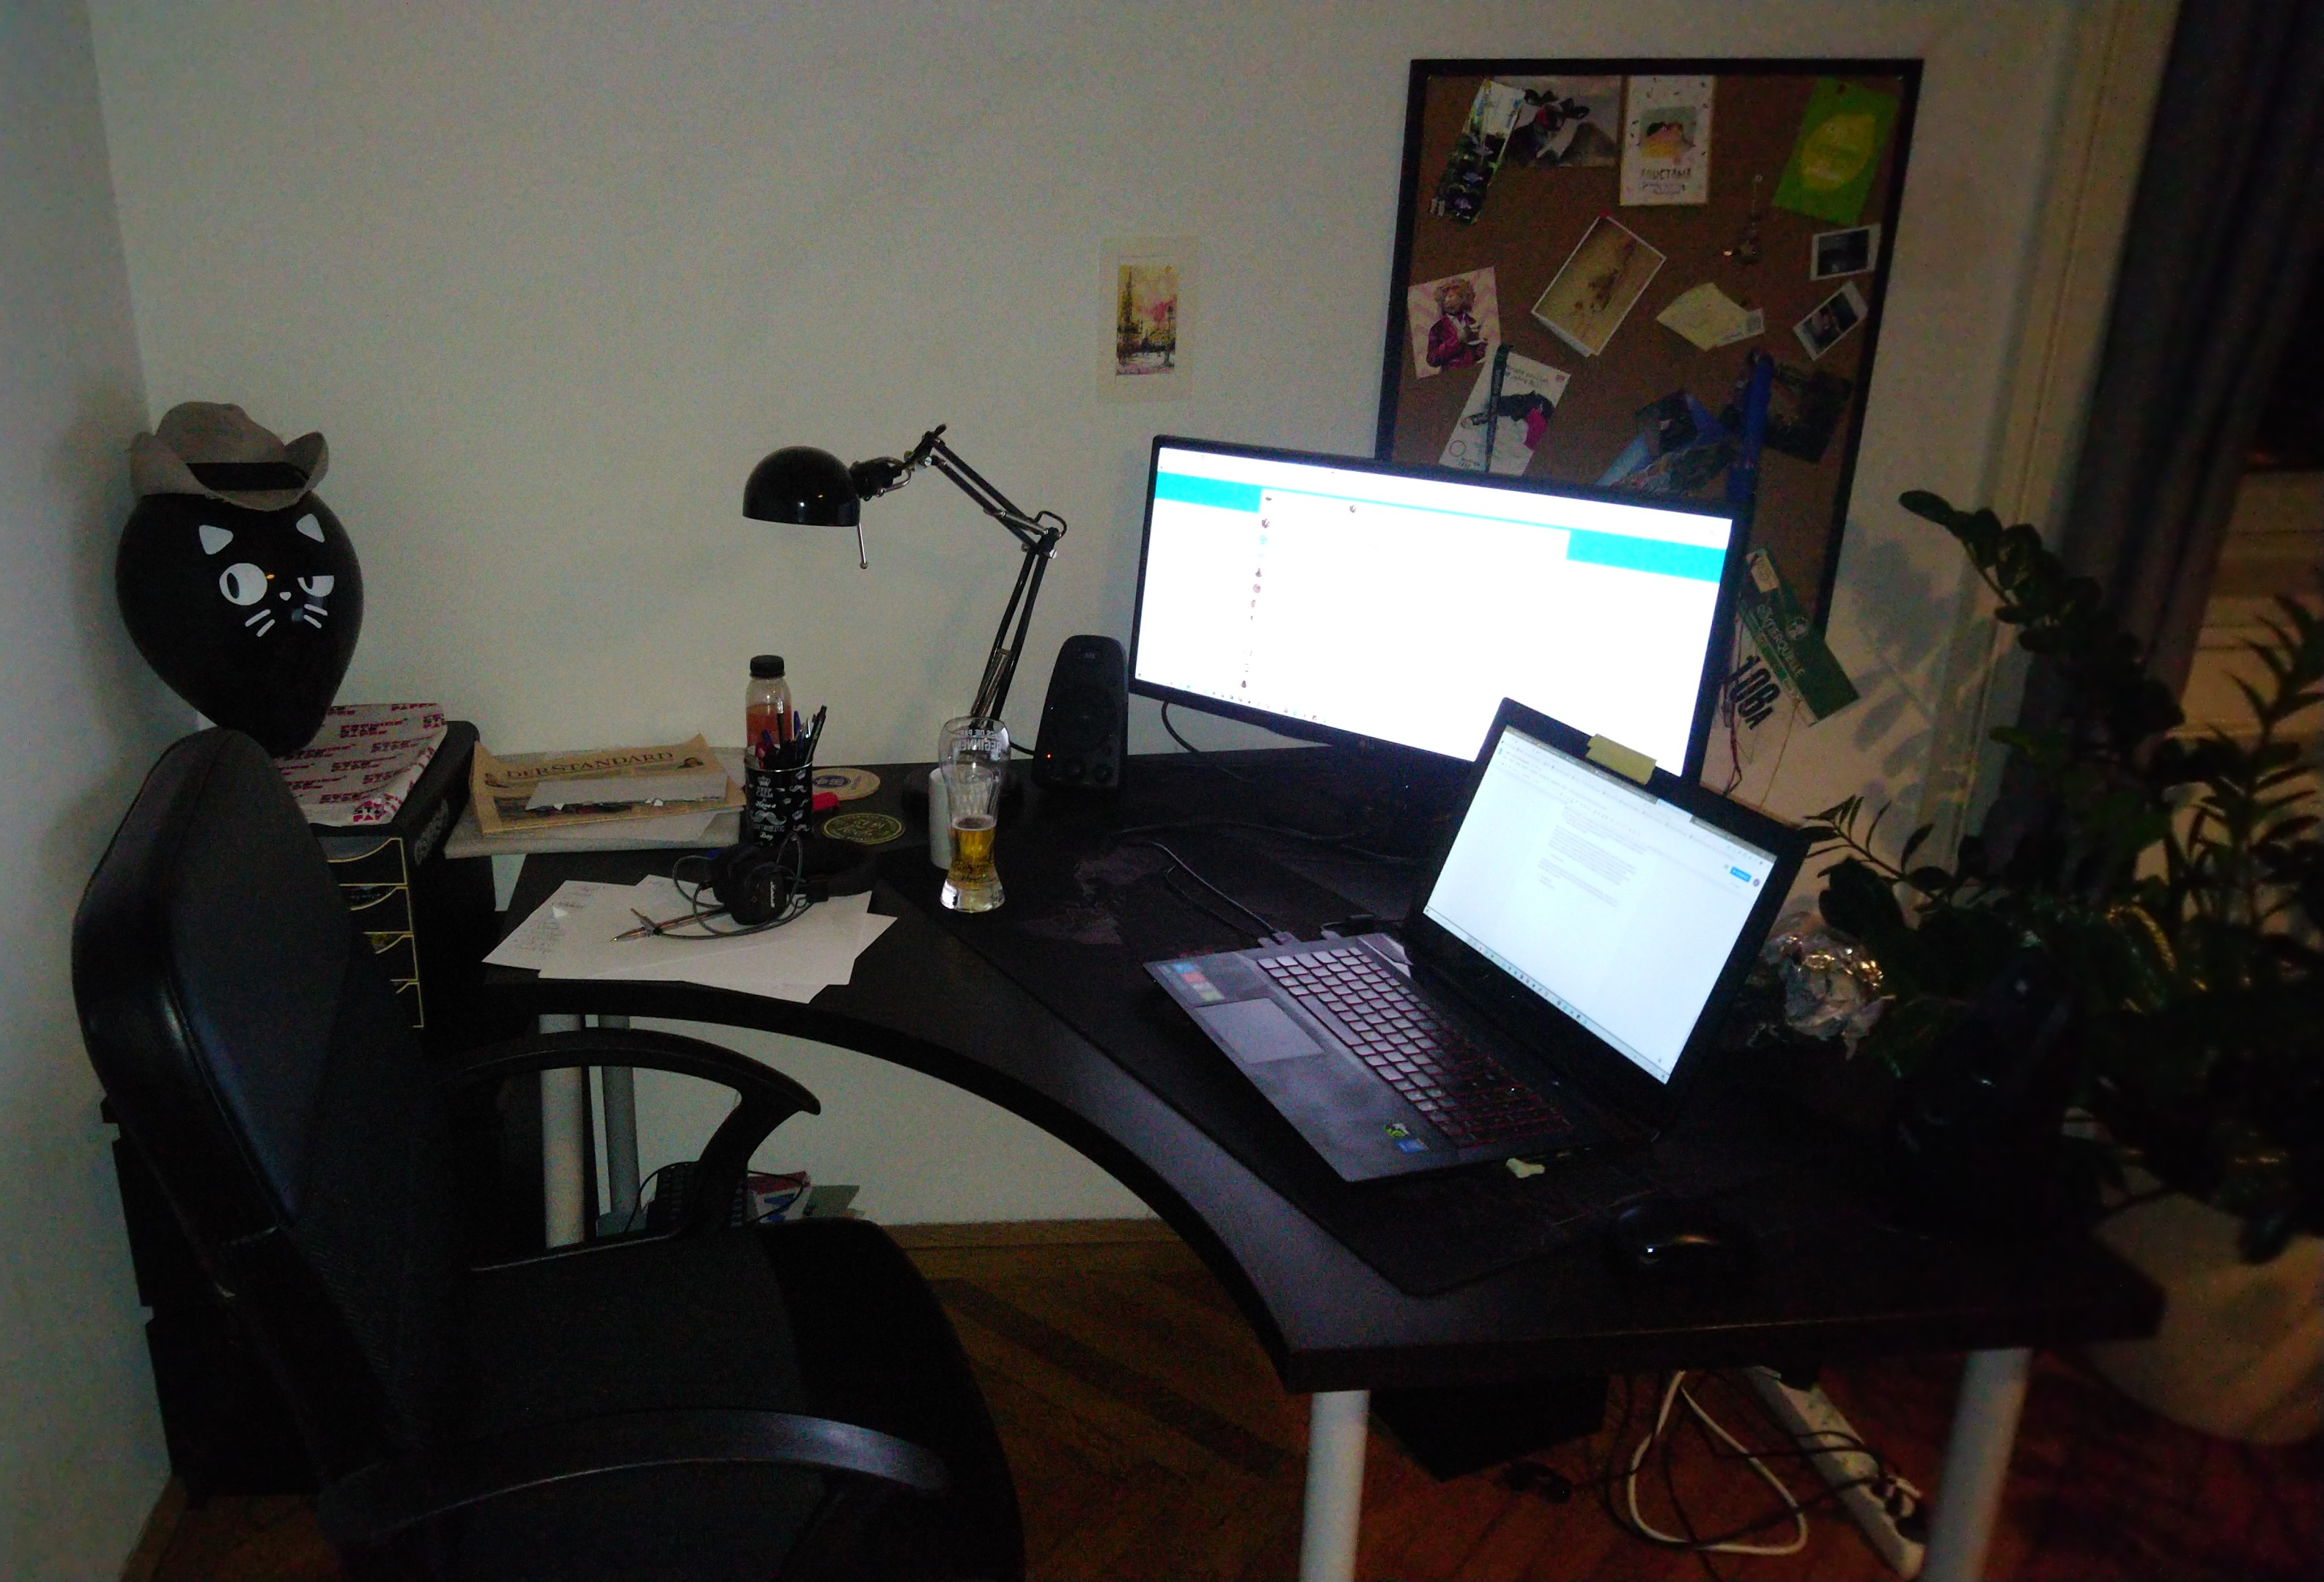
\includegraphics[width=1\columnwidth]{figures/auto-ethnography.JPG}
  \caption{Sample picture from the Auto-Ethnographic method, showing the desk of one of the researchers}~\label{fig:figure1}
\end{figure}

\begin{figure}
\centering
  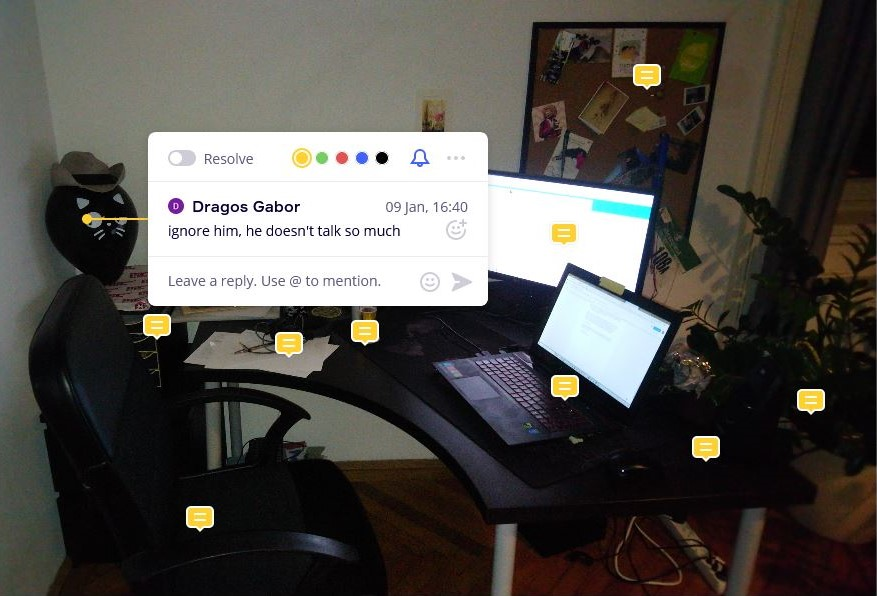
\includegraphics[width=1\columnwidth]{figures/auto-ethnography-annotated.JPG}
  \caption{The same sample picture from the Auto-Ethnographic method, now annotated with small comments from Miro}~\label{fig:figure2}
\end{figure}

\subsubsection{Semi-structured Interviews}
The 5 interview questions
Who were the participants (general information), where the interviews were taken, how we found the participants, age, academic status, consent management, tools, analysing the interview, Miro idea board / extracting data THEMATIC ANALYSING 

Some people did not know how the pandemic will evolve so they did not prepare for a long home learning situation, we asked them how the ideal setup will look like or if they know the next semesters  will be remotely what will they change.

issues: Single interviewer, no observer., subjectivity issues due to the participants being friends

\subsubsection{Photographic Ethnography}
Using the photo analysis method, the researches wanted to discover the study setups of students engaged in distance learning. The method was chosen in order to give a better overview of essential items used by students for improving their health and comfort during online studies, at home. The participants agreed on sending a photo of their environment before the semi-structured online interviews. Moreover, the researchers shared photos of their personal setups used for remote studies. Two consents were used in the research: one sent to the participants before the semi-structured online interview, and another, for the researchers themselves, before starting the auto-ethnography process. The processes of storing, analyzing, anonymizing and deletion of the participants and researchers photos were covered in the mentioned consents.

As visual recording of the personal space can be consider as a breach of privacy, not all the participants agreed to expose their working space. A number of five + (how many Oscar got) photos was collected in the photo analysis process. A visual difference between the state of the learning environment before and after switching to distance learning could not been made, as the photos received by the researchers were taken in the actual context of the pandemic. Only one participant sent photos of their old and their actual setup.  One participant sent a photo of their current setup, and two photos of setups that could serve as inspiration for their ideal setup (see Figure~\ref{fig:figure2}). All photos received by the participants were used in the analyze process.

\begin{figure}
\centering
  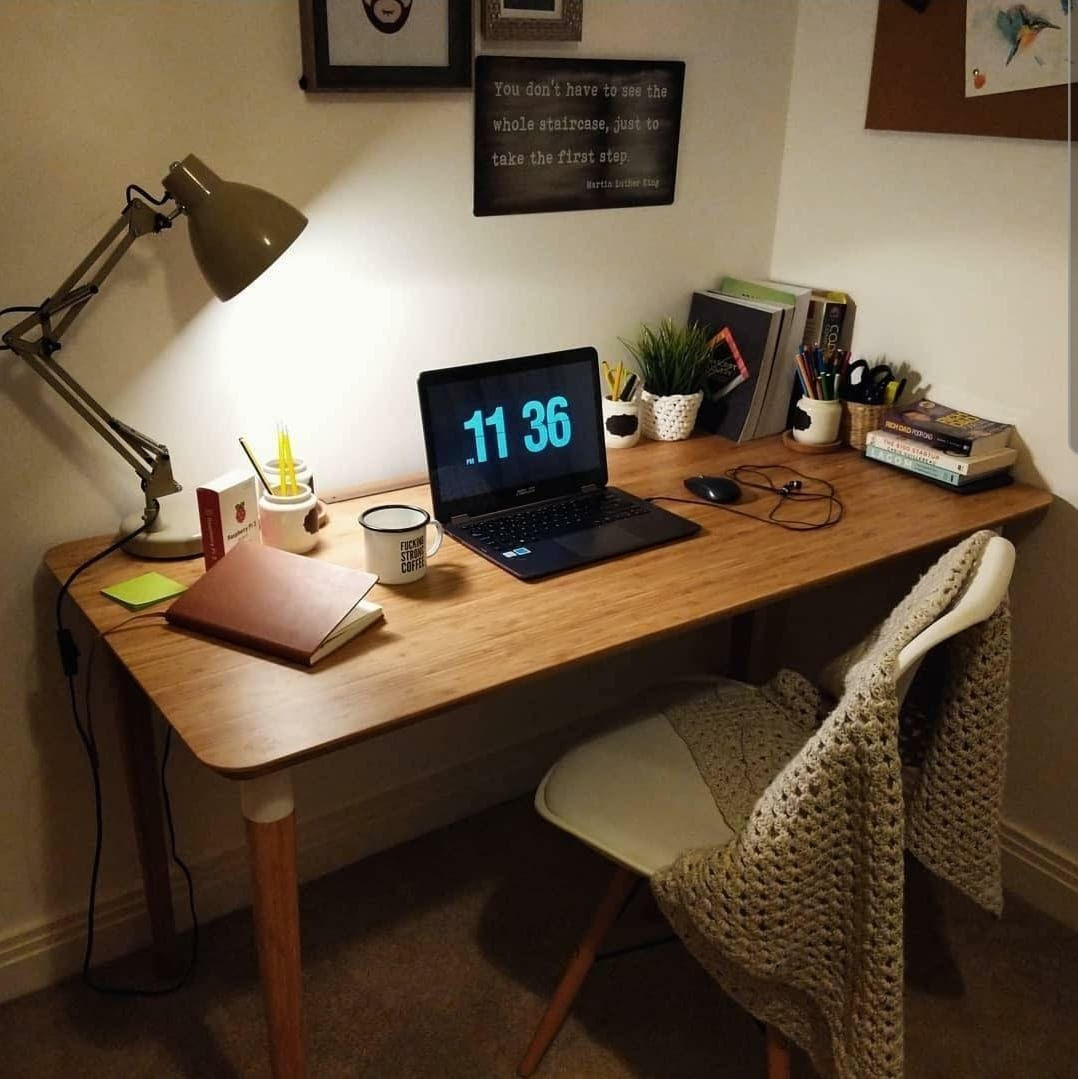
\includegraphics[width=1\columnwidth]{figures/perfect-setup}
  \caption{A sample photo from the Photographic Ethnography method given by one of the participants, it is the desired "perfect study environment''}~\label{fig:figure3}
\end{figure}

\section{Findings}

We need to talk about the research question results here.

Our findings from the interviews

Our findings from the photos: Both participants and from the auto-ethnography 

The analyze of the photos received from the participants and from the researchers involved in the study, showed unique, personalized study environments,  with a commune focus on ergonomics, efficiency and aesthetics. For a better understanding of the students environment, the photo sent by the participants were used as a complementary visualization for the description given in the semi-structured interviews. The result showed that the position of the working desk is usually located close to a direct source of natural light. The importance of a natural source of light was mentioned by several participants during the semi-structured online interview process. Items such as: second screen, laptop, lamp, plants, notebooks were founded present in most of the study setups. The participants explained that the use of a second screen can improve productivity as you can easily multitask when required. When asked about an improvement they would made to the actual setup, participants that were not possessing any additional display mentioned the benefits they would get from owning one.

\section{Discussion}

\subsection{Biases in participation}
There was an obvious variation in the result we achieved. It is therefore feasible to discuss what the research results would have looked like if the number of participants had been higher, or if the participants had studied another educational discipline than engineering. All the participants were students at the Vienna University of Technology in Austria which is a delimitation. Anyway, we believe it was an decent variety of life situations among these participants and thus a representative research overview.
Upon a closer look within the participant’s characteristic, it must be noted that our “sample” is not very diverse from a geographical point of view. All participants, including the researchers themselves live and study either in Austria or another EU member country. In terms of degree, only Bachelors, Masters and PhD students have participated, no lower education. The degree’s have been mostly IT related and both from TU Wien and other European universities as well as Erasmus students

To try to minimize biases in the thematic analysis, all of the participants were renamed to improve an transparent thematic coding. 

However, we argue that unaware biases could still affect the participants behavior and our own interpretations because we knew these students before the research.
A very important bias that had occurred within our interviews is due to the already existing relationships between the researchers and the interview participants as well as the decision of not utilizing the classical interviewer/observer technique due to time constraints as well as the avoidance of causing discomfort towards the participants due to talking about their lives with an unknown person in the interview.

\subsection{Motivation}
But regardless of the participants' background a trend of declining motivation emerged in the research, something we did not plan for. All participants referred several times during the interviews to arguments that they experienced a deteriorating level of motivation despite the fact that we did not ask any semi-structured question about motivation. Motivation can therefore be seen as a rising and hidden problem even if the student's home office equipment or home office studies worked out well. We want to attribute the deteriorating motivation to the prevailing pandemic that forces students to study from home and be isolated from the campus life. What the challenges could entail varied depending on the participants. Two participants clearly stated that they did not appreciate studying without their classmates. One student was missing the sunlight and feeling of freedom. Another student found it difficult to focus on the computer screen during eight hours, but had no big challenges studying remotely. We also saw a pattern that the participants' motivation was stronger in the first semester of the pandemic (2020S) compared with the second semester of the pandemic (2020W).

We believe this can be addressed to the society’s first ignorance of the early pandemic and that people primarily thought the early virus situation would not last for long. We therefore claim that the students' motivation was slightly better during the first semester because they kept their spirits up. This allowed the students to complete their studies in a distance learning format during the first semester of the pandemic without being too negatively affected.

\subsection{Equipment}
This can also be seen as an argument as to why six out of eight participants acquired new technical equipment in the middle of the pandemic, when it was clearer distance learning would continue. Upgrading the home office was eventually considered a necessity now when the students realized that their home office would remain. The technical equipment that was most commonly bought among the participants were extra monitors, touchpads, printers, headphones and mouses. However, we argue that it is still difficult to generalize what type of technical equipment students need to add in their home office setup due to the fact that the setup differs from situations. It can be stated that none of the participants needed to buy a computer to be able to transform into the distance learning format. We believe that this is due to the fact that the university and university studies were already digitized to a large extent before the pandemic broke out. Consequently, as a student switching to full-distance learning was not too painful even though the motivation has been strongly negatively affected. As the technical equipment is central to distance learning, we believe that students in general have chosen to prioritize a decent set-up. We believe that many students prioritize buying the most relevant technical equipment at the beginning of their university education. However, we believe that most students have needed to update some of the technical equipment. Only one of nine participants had for example not bought any extra electrical equipment in 2020. A short conclusion is therefore that most home offices were not optimized for distance learning at the beginning of the pandemic and that many students have had to upgrade their equipment successively.

\subsection{Health and comfort}
Studying in the home office sets a new level of understanding ergonomics depending on the basic office equipment. We would like to point out that there was dissatisfaction with the participants' office chairs, which most have described as being "unergonomic''. The chairs were described as stiff, offered a bad working posture and could not be adjusted in height. We therefore claim that there might be persistent health issues if students do not choose to upgrade their chair in the future home office. Studying at the university offers better ergonomics with chairs, benches and lamps that are adapted for university studies. Consequently, five of the participants answered that they wanted to upgrade their chair if they could. Three of the participants also answered that they would prefer to have a separate office if they could, which is not possible without moving into a new living accommodation. We therefore believe that it is necessary for all students to reflect on their own situation and be flexible and creative in how they can improve their own home office. All students may need different solutions as situations always differ. We also believe that inappropriate routines that office equipment can generate are difficult to detect. It is easy to get used to equipment that works but is not optimal. We therefore urge all students to reflect about their home office standard and how it could be improved. We consider it important to ask the question "what do I need to improve if I am going to study here for a year?". According to the research findings, all participants received some form of negative ergonomics aspect that affected their studies. Good lighting, fresh air or working posture have been the main problems detected. Sitting still in one and the same room was considered as a negative aspect of distance learning. Improving the study area as early as possible, we claim will prevent easy to avoid health issues in the long run.

One of the participants also pointed out that his eyes ached in the evening, after hours in front of the computer. But this can be avoided with regular breaks or blue light-repellent glasses, a solution that the participant did not think about. We believe that this is not because the student does not want to improve his health, but because the student does not prioritize the time of reflecting about the home office setup. We would therefore like to encourage all higher education institutions to offer students a sort of \emph{tips and tricks manual} based on existing research on ergonomics and other desk related comfort improvements in order to better prepare students towards distance learning and gather their attention on the matter.

\subsection{Financial Limitations}
From the fact that participants had difficulty answering questions about their perfect study setup, we argue that they had not processed their own thoughts about whether they could improve their home office or not, which indicates that ergonomics have been prioritized away in the hectic noise of distance learning as well financial limitations. While most of our participants also work, several do not, and one has actually had their job activity interrupted due to the ongoing pandemic restrictions. And so financial limitations have halted their desire of improving their work environment further. Possible partnerships between educational institutions and retailers in order to provide discounts for students could prove effective in cutting costs on behalf of the students and even boost sales for retails, providing a win-win solution. Another solution could be found from the already established furniture rental services, that currently work with other companies in facilitating their move within cities like Vienna, by starting to provide also low to mid end study equipment for Erasmus students.


\section{Implications for design}

It is worth noting that the research presented within this paper is not meant necessarily to provide the HCI community with a new form of interaction or a profoundly new methodological approach in how human-computer interaction can be studied, but it is meant to be seen more through the lens of \cite{dourish_implications_2006} where the significance of \emph{``Implications for design''} stems from observing human habits within a highly isolated scenario where most of the study and work interactions are perpetuated solely through technology. The authors desire is not to emphasize the need for bigger screens, or more comfortable chairs, but to show how much of our lives \emph{can} be replaced through software.

\subsection{Office of the next pandemic}

Given our interviews with the participants, no clear generalizing statement can be drawn on previous study setups possessed before the enactment of social distancing norms. But several have attributed a more aware understanding of the need to have such an environment within their homes. 
Noticing the likely-hood of our current situation to continue for at least one more semester, multiple participants had come to the conclusion and indeed already have plans of improving their study and work environments. Putting in question if a need in providing highly economical solutions in so as to reduce the overall cost of creating such a setup might be the next and most valuable step for the industry to take.

\subsection{Replacement of social interaction}

Multiple participants have expressed an inner desired to talk about their motivational issues while studying in this new environment. And to our amazement, different solutions in coping have been applied by each, from simple \emph{Zoom} study meetups, to arguably illegal (though depending on the country, might not be) face-to-face lecture viewings. Here the authors would like to express that a proper replacement of the in-class lecture experience, still does not exist and some participants have even emphasized a small regress due to the constant gap in interactivity that distance learning cannot overcome.

\section{Conclusions and future work}

1. A study on a more diverse group of students
2. A more in-depth study about motivational aspects
3. West country rich 
4. Didn’t realize the length of the pandemic
5. What could the regulations look like?
6. Maybe (?) we have a OK demographic picture of the participants (students) \\





\section{Acknowledgments}
Thank you to all our interview participants for taking their time off their studies and work in order to help us with this assignment. Thank you to TU Wien for giving us access to the needed tools in order to prepare the assignment, and of course to our supervisory professors for offering us guidance along the way.

% REFERENCES FORMAT
% References must be the same font size as other body text.
\bibliographystyle{SIGCHI-Reference-Format}
\bibliography{sample}

\end{document}

%%% Local Variables:
%%% mode: latex
%%% TeX-master: t
%%% End:
